\section{Quantization}
\label{sec:quantization}

Quantization is the only lossy step. Each subband gets its own uniform scalar quantizer, and
the art of the encoder lies in choosing the bin widths: fine enough in the subbands that
carry ridge structure, coarse enough elsewhere to reach the target bit rate. The quantizer
itself belongs to Part~1 and is the same for every encoder; how the bin widths are chosen is
the business of Part~3.

\subsection{The dead-zone quantizer}

For subband $k$ with bin width $Q_k > 0$ and zero-bin width $Z_k$, a coefficient $a$ is mapped
to the integer index (Annex A.3)
\begin{equation}
  p = \begin{cases}
    \floor{(a - Z_k/2)/Q_k} + 1, & a > Z_k/2,\\
    0, & -Z_k/2 \le a \le Z_k/2,\\
    \ceil{(a + Z_k/2)/Q_k} - 1, & a < -Z_k/2,
  \end{cases}
  \label{eq:quantize}
\end{equation}
and the decoder maps it back to
\begin{equation}
  \hat a = \begin{cases}
    (p - C)\,Q_k + Z_k/2, & p > 0,\\
    0, & p = 0,\\
    (p + C)\,Q_k - Z_k/2, & p < 0.
  \end{cases}
  \label{eq:dequantize}
\end{equation}
Figure~\ref{fig:quantizer} shows the bins. The zero bin is wider than the others
($Z_k = 1.2\,Q_k$ in encoder number two), a \emph{dead zone} that sends more of the many small
coefficients to zero; zeros are what the entropy coder compresses best, since it codes runs of
them with a single symbol. The parameter $C$ sets where in its bin a nonzero index is
reconstructed. Encoder number two uses $C = 0.44$, which puts $\hat a$ at $0.56\,Q_k$ from the
inner edge of the bin, slightly beyond its middle. A bin width $Q_k = 0$ means that subband $k$
is not transmitted at all: the decoder sets all its coefficients to zero.

\begin{figure}[ht]
  \centering
  \begin{tikzpicture}[x=1cm,y=1cm,font=\small]
  % Z = 2.4, Q = 2 (Z = 1.2 Q); C = 0.44
  \def\Zh{1.2}\def\Q{2}\def\C{0.44}
  \draw[->] (-6.6,0) -- (6.9,0) node[right] {$a$};
  % bin edges
  \foreach \s in {-1,1} {
    \foreach \i in {0,1,2} {
      \pgfmathsetmacro{\e}{\s*(\Zh+\i*\Q)}
      \draw (\e,-0.18) -- (\e,0.18);
    }
  }
  \node[below=1mm,font=\footnotesize] at (\Zh,-0.12) {$\tfrac{Z}{2}$};
  \node[below=1mm,font=\footnotesize] at (-\Zh,-0.12) {$-\tfrac{Z}{2}$};
  \node[below=1mm,font=\footnotesize] at (\Zh+\Q,-0.12) {$\tfrac{Z}{2}{+}Q$};
  \node[below=1mm,font=\footnotesize] at (-\Zh-\Q,-0.12) {$-\tfrac{Z}{2}{-}Q$};
  % indices
  \node at (0,0.55) {$p=0$};
  \foreach \i in {1,2} {
    \pgfmathsetmacro{\c}{\Zh+(\i-0.5)*\Q}
    \node at (\c,0.55) {$p=\i$};
    \node at (-\c,0.55) {$p=-\i$};
  }
  \node at (6.1,0.55) {$\cdots$};
  \node at (-6.1,0.55) {$\cdots$};
  % reconstruction points (p - C) Q + Z/2
  \foreach \i in {1,2} {
    \pgfmathsetmacro{\r}{(\i-\C)*\Q+\Zh}
    \fill (\r,0) circle (0.07);
    \fill (-\r,0) circle (0.07);
  }
  \fill (0,0) circle (0.07);
  % braces
  \draw[decorate,decoration={brace,amplitude=4pt,mirror}] (-\Zh,-0.75) -- (\Zh,-0.75)
    node[midway,below=4pt,font=\footnotesize] {zero bin, width $Z$};
  \draw[decorate,decoration={brace,amplitude=4pt,mirror}] (\Zh+\Q,-0.75) -- (\Zh+2*\Q,-0.75)
    node[midway,below=4pt,font=\footnotesize] {width $Q$};
  \pgfmathsetmacro{\ra}{(1-\C)*\Q+\Zh}
  \draw[densely dotted] (\ra,0) -- (\ra,-1.55) node[below,font=\footnotesize] {$\hat a = (1-C)\,Q + \tfrac{Z}{2}$};
\end{tikzpicture}

  \caption{The dead-zone scalar quantizer with $Z = 1.2\,Q$. Dots mark the reconstruction
  values for $C = 0.44$.}
  \label{fig:quantizer}
\end{figure}

\subsection{Subband variances}
\label{sec:variance}

Encoder number two chooses the bin widths from the variance of each subband. Fingerprints
rarely fill the scanned area, and the background around them would make the variances
unrepresentative, so the variance is normally estimated on a central window of each subband
(Part 3, Section 3.1). For a subband of $X_k \times Y_k$ coefficients the window has
\begin{equation}
  X'_k = \floor{3X_k/4} \text{ columns starting at } \floor{X_k/8}, \qquad
  Y'_k = \floor{7Y_k/16} \text{ rows starting at } \floor{9Y_k/32},
  \label{eq:window}
\end{equation}
as in Figure~\ref{fig:window}: up to rounding, the window is centred and covers three quarters
of the width and seven sixteenths of the height. The variance is the unbiased estimate over the
window,
\begin{equation}
  \sigma_k^2 = \frac{1}{X'_kY'_k - 1}\sum_{m,n \in \text{window}} \bigl(a_k(m,n) - \mu_k\bigr)^2,
  \label{eq:variance}
\end{equation}
where $\mu_k$ is the mean over the window.

\begin{figure}[ht]
  \centering
  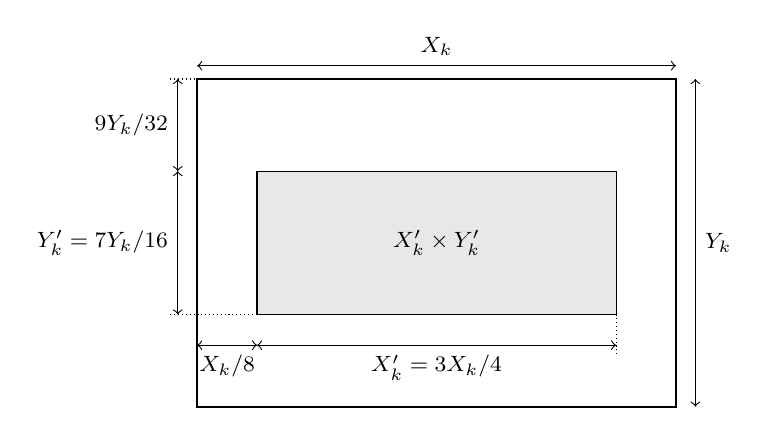
\begin{tikzpicture}[x=0.19cm,y=-0.13cm,font=\footnotesize]
  % subband of 32 x 32 units; window x0 = X/8 = 4, width 3X/4 = 24; y0 = 9Y/32 = 9, height 7Y/16 = 14
  \draw[line width=0.7pt] (0,0) rectangle (32,32);
  \fill[gray!18] (4,9) rectangle (28,23);
  \draw (4,9) rectangle (28,23);
  \node at (16,16) {$X'_k \times Y'_k$};
  \draw[<->] (0,-1.3) -- node[above] {$X_k$} (32,-1.3);
  \draw[<->] (33.3,0) -- node[right] {$Y_k$} (33.3,32);
  \draw[<->] (0,26) -- node[below] {$\floor{X_k/8}$} (4,26);
  \draw[<->] (4,26) -- node[below] {$X'_k = \floor{3X_k/4}$} (28,26);
  \draw[<->] (-1.3,0) -- node[left] {$\floor{9Y_k/32}$} (-1.3,9);
  \draw[<->] (-1.3,9) -- node[left] {$Y'_k = \floor{7Y_k/16}$} (-1.3,23);
  \draw[densely dotted] (0,26) -- (0,32) (28,23) -- (28,27);
  \draw[densely dotted] (-1.8,0) -- (0,0) (-1.8,23) -- (4,23);
\end{tikzpicture}

  \caption{The window used to estimate the variance of a subband.}
  \label{fig:window}
\end{figure}

Version~3.1 of the specification added a safeguard, and this is the whole difference between
encoder number one and encoder number two. Live-scan devices with 3-inch platens capture two
thumbs side by side, and when the thumbs rest near the bottom edge they fall outside the
window. The window variances then describe the background rather than the prints, the bin
widths are chosen badly, and in extreme cases every print is lost from the decoded image
\cite{nistnotice}. The fix tests the
four lowest-frequency subbands: if
\begin{equation}
  \sigma_0^2 + \sigma_1^2 + \sigma_2^2 + \sigma_3^2 > 20\,000
\end{equation}
with the window estimates, the window is used for every subband; otherwise every variance is
recomputed over the whole subband ($X'_k = X_k$, $Y'_k = Y_k$, starting at the corner). NIST
reports that about 12\% of two-thumb images switch to the full region, and fewer than 0.5\% of
other impressions do. In the NIST compliance set, 7 of the 40 images do.

\subsection{Bin widths}
\label{sec:binwidths}

The bin widths come from a classical bit-allocation argument \cite{bradley1993}. Assume that the
coefficients of subband $k$ lie in an interval of $2\gamma$ standard deviations,
$[\mu_k - \gamma\sigma_k, \mu_k + \gamma\sigma_k]$ with \emph{loading factor} $\gamma = 2.5$.
(Outliers do no harm, because the entropy coder handles them with escape codes.) A quantizer
with bin width $Q_k$ then has $L_k = 2\gamma\sigma_k/Q_k$ bins and spends
$r_k = \log_2 L_k$ bits per coefficient. Subband $k$ has $XY/m_k$ coefficients, so the average
rate over the image is
\begin{equation}
  r = \sum_{k \in K} \frac{r_k}{m_k} = \sum_{k \in K} \frac{1}{m_k}\log_2\frac{2\gamma\sigma_k}{Q_k}
  \quad\text{bits per pixel},
  \label{eq:rate}
\end{equation}
where $K$ is the set of subbands that receive bits. This is the constraint; the remaining
freedom is the \emph{relative} widths. Encoder number two fixes them as
\begin{equation}
  Q_k = Q'_k / q, \qquad
  Q'_k = \begin{cases}
    1, & 0 \le k \le 3,\\
    \dfrac{10}{A_k \ln \sigma_k^2}, & 4 \le k \le 59,\\
    0, & 60 \le k \le 63 \text{ or } \sigma_k^2 < 1.01,
  \end{cases}
  \qquad Z_k = 1.2\,Q_k,
  \label{eq:relwidths}
\end{equation}
with weights $A_k = 1.32$ for $k \in \{52, 56\}$, $1.08$ for $k \in \{53, 55, 58, 59\}$,
$1.42$ for $k \in \{54, 57\}$, and $1$ otherwise. The logarithm makes high-variance subbands
(the ones with ridge structure) get finer bins, the weights fine-tune the quarter-size
subbands, and subbands with almost no variance are dropped. The single constant $q$ scales all
widths together. Substituting $Q_k = Q'_k/q$ into Equation~\eqref{eq:rate} and writing
$S = \sum_{k\in K} 1/m_k$ for the fraction of coefficients that receive bits gives
$r = S\log_2(2\gamma q) + \sum_{k\in K} m_k^{-1}\log_2(\sigma_k/Q'_k)$, and solving for $q$,
\begin{equation}
  q = \frac{2^{r/S - 1}}{\gamma}\,
      \Biggl[\,\prod_{k\in K}\Bigl(\frac{\sigma_k}{Q'_k}\Bigr)^{1/m_k}\Biggr]^{-1/S}.
  \label{eq:q}
\end{equation}

One complication remains. If a subband's bin turns out wider than its whole range,
$Q_k \ge 2\gamma\sigma_k$, the model gives it a negative rate $r_k$, which is meaningless and
would let the other subbands overspend. Such subbands are removed from $K$ and $q$ is
recomputed, until no subband is left with a nonpositive rate (Algorithm~\ref{alg:binwidths}).
The removed subbands are still quantized with the final widths: they are expected to quantize
almost entirely to zero, but the few coefficients that survive are kept.

\begin{algorithm}[ht]
  \caption{Bin widths of encoder number two (Part 3, Section 3.2).}
  \label{alg:binwidths}
  \begin{algorithmic}[1]
    \Require subband variances $\sigma_k^2$ ($k = 0..59$); target rate $r$ in bits per pixel; $\gamma = 2.5$
    \Ensure bin widths $Q_k$ and $Z_k$ for $k = 0..63$
    \State compute $Q'_k$ by Eq.~\eqref{eq:relwidths}
    \State $K_0 \gets \{k \le 59 : \sigma_k^2 \ge 1.01\}$;\ $K \gets K_0$
    \Loop
      \State $S \gets \sum_{k\in K} 1/m_k$
      \State $q \gets \gamma^{-1}\, 2^{r/S - 1} \bigl[\prod_{k\in K} (\sigma_k/Q'_k)^{1/m_k}\bigr]^{-1/S}$
      \State $\Xi \gets \{k \in K : Q'_k/q \ge 2\gamma\sigma_k\}$ \Comment{nonpositive rates}
      \If{$\Xi = \emptyset$} \textbf{break} \EndIf
      \State $K \gets K \setminus \Xi$
    \EndLoop
    \For{$k \gets 0$ \textbf{to} $63$}
      \State $Q_k \gets Q'_k/q$ \textbf{if} $k \in K_0$ \textbf{else} $0$;\quad $Z_k \gets 1.2\,Q_k$
    \EndFor
  \end{algorithmic}
\end{algorithm}

The rate $r$ is only a target, since the model ignores how the entropy coder actually behaves.
On the 40 images of the NIST compliance set, the NIST encoder asked for $r = 0.75$ produced
files of 0.53 bits per pixel on average (from 0.19 to 0.75, counting the whole file), and
asked for $r = 2.25$, files of 1.66 bits per pixel (from 0.35 to 2.31).
